% +--------------------------------------------------------------------+
% | Sample Chapter 1
% |
% | This file provides examples of how to
% | - insert a figure with a caption
% | - construct a table with a caption
% | - create subsections within the chapter
% | - insert a reference to a Figure or Table
% | - make a citation
% +--------------------------------------------------------------------+

\cleardoublepage

% +--------------------------------------------------------------------+
% | Replace "Chapter Title" below with the title of your chapter.
% | LaTeX will automatically number the chapters.
% +--------------------------------------------------------------------+

\chapter{Introduction to Leibniz-type rules}\label{chapter1}
\label{makereference1}

Fractional Leibniz rules have been extensively studied due to their connections to partial differential equations that model many real world situations such as shallow water waves and fluid flow. In this chapter, we introduce the subject of Leibniz-type rules and describe the main results to be discussed in Chapters \ref{chapter2} and \ref{chapter3} of this dissertation.


First consider the Leibniz rule taught in Calculus courses, which expresses the derivatives of a product of functions as a linear combination of derivatives of the functions involved; more specifically, for functions $f$ and $g$ sufficiently smooth, it holds that
\[\partial^\alpha (fg)(x) = \sum_{\beta \leq \alpha} \binom{\alpha}{\beta} \partial^{\alpha - \beta} f(x) \partial^{\beta} g(x) = \partial^\alpha f(x) g(x) + f(x) \partial^\alpha g(x) + \cdots ,\]
for $\alpha,\beta \in \mathbb{N}^n_0$.
In an analogous way, fractional Leibniz rules give estimates of the smoothness and size of a product of functions in terms of the smoothness and size of the factors. For instance, for $f$ and $g$ in the Schwartz class $\mathcal{S}(\mathbb{R}^n)$, it holds that
\begin{equation}\label{def:leibniz}
\norm{D^s (fg)}{L^p} \lesssim \norm{D^s f}{L^{p_1}}\norm{g}{L^{p_2}} + \norm{f}{L^{\tilde{p}_1}}\norm{D^s g}{L^{\tilde{p}_2}},
\end{equation}
where $1/p = 1/p_1 + 1/p_2 =  1/\tilde{p}_1 + 1/\tilde{p}_2$, $1\leq p_1,p_2,\tilde{p}_1,\tilde{p}_2\leq \infty$, $1/2 \leq p\leq \infty$, $s>n(1/\text{min}(p,1) - 1)$ or $s$ is an even whole number, and $L^r$ denotes a Lebesgue space for $0<r\leq \infty$. The homogeneous fractional differentiation operator of order $s$, $D^s$, is defined as \[D^s f(x) = \int_\rn |\xi|^s \widehat{f}(\xi) e^{2\pi i x\cdot \xi} d\xi,\]
where $\widehat{f}$ is the Fourier transform of $f$.
For $s>0$, the operator $D^s$ is naturally understood as taking $s$ derivatives of its argument. Indeed, in the case $s=2$, $D^2f = \frac{-1}{4\pi^2}\Delta f$, where $\Delta = \sum_{j=1}^n \partial^2_{x_j}$ is the Laplacian operator. Furthermore, if $s$ is a positive integer and $1<p<\infty$,

%the $\dot{W}^{k,p}$ norm and $\norm{D^k \cdot}{L^p}$ are equivalent norms where 
%\[\norm{f}{\cdot{W}^{k,p}} = \sum_{|\alpha|=k} \norm{\partial^\alpha}{L^p}.\] 

\[\norm{D^s f}{L^p} \sim \sum_{|\alpha| = s} \norm{\partial^\alpha f}{L^p},\]
where $|\alpha| = \alpha_1 + \alpha_2 + ... + \alpha_n$ for $\alpha = (\alpha_1,\alpha_2,...,\alpha_n) \in \mathbb{N}^n_0.$

 Another version of (\ref{def:leibniz}) is obtained by using the inhomogeneous $s$th order fractional differentiation operator $J^s$:
\begin{equation}\label{def:ileibniz}
\norm{J^s(fg)}{L^p} \lesssim \norm{J^s f}{L^{p_1}}\norm{g}{L^{p_2}} + \norm{f}{L^{\tilde{p}_1}}\norm{J^s g}{L^{\tilde{p}_2}},
\end{equation}
where $p_1,p_2,\tilde{p}_1, \tilde{p}_2,$ and $s$ satisfy the same conditions as for (\ref{def:leibniz}).
Similarly to its homeogenous counterpart, the operator $J^s$ is defined through the Fourier transform as 
\[ J^s f(x) = \int_{\rn} (1+|\xi|^2)^\frac{s}{2} \widehat{f}(\xi)e^{2\pi i x\cdot\xi} d\xi\]
and can be interpreted as taking derivatives up to order $s$ of $f$ when $s>0$.
%Then $s>0$ it is interpreted as taking up to $s$ derivatives of the function it is applied to as when $s=k$ is a positive integer $\norm{J^k(f)}{L^p} = \norm{f}{W^{k,p}}$ where $\norm{f}{W^{k,p}} = \sum_{|\alpha|\leq k} \norm{\partial^\alpha f}{L^p}$.


The estimates (\ref{def:leibniz}) and (\ref{def:ileibniz}) are also known as Kato-Ponce inequalities due to the foundational work of Kato-Ponce \cite{MR951744}, where the estimate (\ref{def:ileibniz}) was proved in the case $1<p=p_1=\tilde{p}_2<\infty$ and $p_2=\tilde{p}_1=\infty$, with applications to the Cauchy problem for Euler and Navier-Stokes equations. This result was extended by Gulisashvili-Kon \cite{MR1420922}, who showed (\ref{def:leibniz}) and (\ref{def:ileibniz}) for the cases $s>0$, $1<p<\infty$, and $1 < p_1,p_2,\tilde{p}_1,\tilde{p}_2\leq\infty$ in connection to smoothing properties of Schr\"odinger semigroups. Grafakos-Oh \cite{MR3200091} and Muscalu-Schlag \cite{MR3052499} established the cases for $1/2 <p\leq 1$; the case $p=\infty$ was completed in the work of Bourgain-Li \cite{MR3263081} and Grafakos-Maldonado-Naibo \cite{MR3189525}; finally, the case $p_1 = 1$, $1\leq p_2 \leq \infty$ and $\frac{1}{2} \leq p \leq 1$ was established by Oh-Wu \cite{Oh_Wu}. Applications of the estimates (\ref{def:leibniz}) and (\ref{def:ileibniz}) to Korteweg-de Vries equations were studied by Christ-Weinstein \cite{MR1124294} and Kenig-Ponce-Vega \cite{MR1211741}.

In the estimates (\ref{def:leibniz}) and (\ref{def:ileibniz}), the two functions $f$ and $g$ are related through pointwise multiplication. In this dissertation, we will consider bilinear estimates in the spirit of (\ref{def:leibniz}) and (\ref{def:ileibniz}) where the two functions are related through a pseudodifferential operator. Let $\sigma(x,\xi,\eta)$ be a smooth, complex-valued function defined for $x,\xi,\eta\in\rn$. We define the \textit{bilinear pseudodifferential operator}  associated to $\sigma$, $T_\sigma$, by 
\begin{equation}\label{psydo}
T_{\sigma}(f,g)(x) = \int_{\mathbb{R}^{2n}} \sigma(x,\xi,\eta) \widehat{f}(\xi)\widehat{g}(\eta)e^{2\pi i x\cdot(\xi+\eta)}d\xi d\eta. 
\end{equation}

\noindent We call $\sigma$ the \textit{symbol} of the operator $T_\sigma$; when $\sigma$ is independent of $x$, $\sigma$ is also referred to as the \textit{multiplier} of the \textit{bilinear multiplier operator} $T_\sigma$. We note that $\sigma \equiv 1$ gives $T_\sigma(f,g) = fg$. 


In Chapters \ref{chapter2} and \ref{chapter3} we will present new results on Leibniz-type rules associated to bilinear pseudodifferential operators that are of the form 
\begin{equation}\label{h_general_estimate}
\norm{D^s T_\sigma(f,g)}{Z} \lesssim \norm{D^sf}{X_1}\norm{g}{Y_1} + \norm{f}{X_2}\norm{D^s g}{Y_2} ,
\end{equation}
\begin{equation}\label{i_general_estimate}
\norm{J^sT_\sigma(f,g)}{Z} \lesssim \norm{J^sf}{X_1}\norm{g}{Y_1} + \norm{f}{X_2}\norm{J^sg}{Y_2} ,
\end{equation}
for a variety of function spaces $X_1$, $X_2$, $Y_1$, $Y_2$, and $Z$. In the particular case that $\sigma \equiv 1$ and $X_1$, $X_2$, $Y_1$, $Y_2$, and $Z$ are appropriate Lebesgue spaces, (\ref{h_general_estimate}) and (\ref{i_general_estimate}) recover (\ref{def:leibniz}) and (\ref{def:ileibniz}) respectively. The main results presented in Chapter \ref{chapter2} will appear in Naibo-Thomson \cite{NaTh_CM}, while those discussed in Chapter \ref{chapter3} were published in Naibo-Thomson \cite{MR3912862}.

In Chapter \ref{chapter2}, we will discuss Leibniz-type rules (\ref{h_general_estimate}) and (\ref{i_general_estimate}) in the setting of Besov and Triebel-Lizorkin spaces based on certain quasi-Banach spaces. Such bilinear estimates will be proved for bilinear Coifman-Meyer multiplier operators. A particular case of the results in Chapter \ref{chapter2} is the following fractional Leibniz rule, and its inhomogeneous counterpart, in the context of Hardy spaces:
\begin{equation}\label{KP:Hardy}
\norm{D^s(fg)}{H^p} \lesssim \norm{D^s f}{H^{p_1}} \norm{g}{H^{p_2}} +  \norm{f}{H^{\tilde{p}_1}}   \norm{D^s g}{H^{\tilde{p}_2}}, 
\end{equation}
where $0<p,p_1, p_2,\tilde{p}_1, \tilde{p}_2 <\infty$ and $1/p = 1/p_1 + 1/p_2 = 1/\tilde{p}_1 + 1/\tilde{p}_2$. Recalling that $H^p = L^p$ for $1<p<\infty$, (\ref{KP:Hardy}) extends and improves (\ref{def:leibniz}). Indeed, the inequality \eqref{KP:Hardy} extends the range of $p$, $p_1$, $p_2$, $\tilde{p}_1$, $\tilde{p}_2$ by allowing $0<p,p_1,p_2,\tilde{p}_1,\tilde{p}_2<\infty$, while \eqref{def:leibniz} requires $1<p_1,p_2,\tilde{p}_1, \tilde{p}_2\leq \infty$. Additionally, (\ref{KP:Hardy}) allows for the $H^p$ norm on the left-hand side, which is larger than the $L^p$ norm. 
  
The techniques used in the proofs of the results in Chapter \ref{chapter2} are quite flexible and allow us to obtain \eqref{h_general_estimate} and \eqref{i_general_estimate} in Triebel-Lizorkin and Besov spaces based on weighted Lebesque spaces, weighted Lorrentz spaces, weighted Morrey spaces, and variable-exponent Lebesgue spaces.
In particular, the proofs make use of Nikol'ski\u\i$\text{ }$  representations of such function spaces. These representations have been used in unweighted settings in the work of Nikol'ski\u\i$\text{ }$  \citep{MR0374877}, Meyer \citep{MR639462}, Bourdad \citep{MR673825}, Triebel \citep{MR3024598}, and Yamazaki \citep{MR837335}. 

As an application of the results in Chapter \ref{chapter2} we obtain scattering properties for solutions to certain systems of partial differential equations that involve fractional powers of the Laplacian. Solutions of these systems scatter to functions that can be realized in terms of a Coifman-Meyer multiplier operator acting on appropriate arguments. As a consequence, the main results of Chapter \ref{chapter2} can be applied and lead to estimates associated to the long term behavior of the solutions. 

In Chapter \ref{chapter3}, we present Leibniz-type rules in Besov and local Hardy spaces for bilinear pseudodifferential operators associated to symbols in bilinear H\"ormander classes of critical order. For such symbols we prove bilinear estimates of the form 

\begin{equation}
\norm{J^s T_\sigma(f,g)}{B^0_{p,q}} \lesssim \norm{J^s f}{B^0_{p_1,q}} \norm{g}{h^{p_2}} + \norm{f}{h^{p_1}}\norm{J^s g}{B^0_{p_2,q}},
\end{equation}
where $B^0_{p,q}$ and $h^p$ denote Besov and local Hardy spaces respectively, $0<p<\infty$ and $0<p_1,p_2\leq\infty$ are such that $1/p = 1/p_1 + 1/p_2$, $0<q\leq\infty$ and $s>n(1/\text{min}(p,1) - 1)$.

%\begin{theorem}\label{thm:critical_besov}
%Let $0<p<\infty$ and $0<p_1,p_2\leq\infty$ be such that $1/p = 1/p_1 + 1/p_2$, $0<q\leq\infty$, $s>\text{max}\{0,n(1/p - 1)\}$, and $0\leq \delta\leq \rho <1$. If $\sigma\in BS^{m(\rho,p_1,p_2)}_{\rho,\delta}$ then it holds that 
%\begin{equation}\label{critical_est}
%\norm{T_\sigma(f,g)}{B^s_{p,q}} \lesssim \norm{f}{B^s_{p_1,q}} \norm{g}{h^{p_2}} + \norm{f}{h^{p_1}}\norm{g}{B^s_{p_2,q}} \quad \forall f,g\in\mathcal{S}(\rn),
%\end{equation}
%where $h^{p_1}$ and $h^{p_2}$ must be replaced by $L^\infty$ if $p_1 = \infty$ or $p_2 = \infty$ respectively. 
%\end{theorem}

%Boundedness properties of bilinear pseudodifferential operators with symbols
%in the bilinear H\"ormander classes have been extensively studied in the settings of
%Lebesgue and Hardy spaces; see B\'enyi-Bernicot-Maldonado-Naibo-Torres \citep{MR2660466}, B\'enyi-Chaffee-Naibo \citep{benyi2018strongly}, B\'enyi-Maldonado-Naibo-Torres \citep{MR1986065}, MR2660466}, Brummer-Naibo \citep{MR3750234}, Herbert-Naibo \citep{MR3627725}, \citep{MR3211086}], Koezuka-Tomita \citep{MR3750316}, Michalowski-Rule-Staubach \citep{MR3165300}, Miyachi-Tomita
%\citep{MR3179688, MT1, MT2}, Naibo \cite{MR3393696, MR3411149}, Rodr\'iguez-L\'opez-Staubach \citep{MR3035059}, and the references therein.

The proofs of the results in Chapter \ref{chapter3} utilize appropriate spectral decompositions of the symbols, pointwise inequalities in terms of maximal functions, and Nikol'ski\u\i$\text{ }$  representations for Besov spaces. The techniques used are inspired by bilinear techniques used in Naibo \cite{MR3393696} and techniques for linear operators in Johnsen \citep{MR2163627}, Marschall \citep{MR1376592}, and Park \citep{Park}. 
%Results related to estimate \ref{critical_est} were proved for the forbidden class $BS^0_{1,1}$ in Koezuka-Timita \cite{MR3750316} and Naibo \citep{MR3393696}. Concerning bilinear pseudodifferential operators with symbols belonging to the subcritical classes $BS^m_{\rho,\delta}$ with $m<m(\rho,p_1,p_2)$ and $1\leq p_1,p_2,p \leq \infty$ ($1 < p_1,p_2,p < \infty$ when $\rho = \delta = 0$) estimate \ref{critical_est} was shown in Naibo \citep{MR3393696} Theorem 1.3. Theorem \ref{thm:critical_besov} extends this result to the critical classes and allows for the indices to be in the wider range $(0,\infty)$. 

We close this chapter by referencing serveral works in connection with the study of the bilinear estimates \eqref{h_general_estimate} and \eqref{i_general_estimate}. In \cite{MR3750234}, Brummer-Naibo studied Leibniz-type rules for bilinear pseudodifferential operators with homogeneous symbols and in function spaces that admit a molecular decomposition and a $\varphi$-transform characterization in the sense of Frazier-Jawerth \cite{MR808825, MR1070037}. In the context of Lebesgue spaces and mixed Lebesgue spaces, estimates of the type (\ref{h_general_estimate}) were studied in Hart-Torres-Wu \cite{MR3864388} for bilinear multiplier operators with minimal smoothness assumptions on the multipliers. Related mapping properties for bilinear pseudodifferential operators with symbols in the bilinear H\"ormander classes were studied by B\'enyi-Torres \cite{MR1986065} and B\'enyi-Nahmod-Torres \cite{MR2250054} in the setting of Sobolev spaces, by B\'enyi \cite{MR1996120} in the setting of Besov spaces, and by Naibo \cite{MR3393696} and Koezuka-Tomita \cite{MR3750316} in the context of Triebel-Lizorkin spaces. Additionally, versions of (\ref{def:leibniz}) and (\ref{def:ileibniz}) in weighted Lebesgue spaces were proved in Cruz-Uribe-Naibo \cite{MR3513582}, while Brummer-Naibo \cite{BrNa2017} proved (\ref{h_general_estimate}) and (\ref{i_general_estimate}) in weighted Lebesgue spaces for Coifman-Meyer multiplier operators. 


%\begin{figure}[htb]%t=top, b=bottom, h=here
%
%    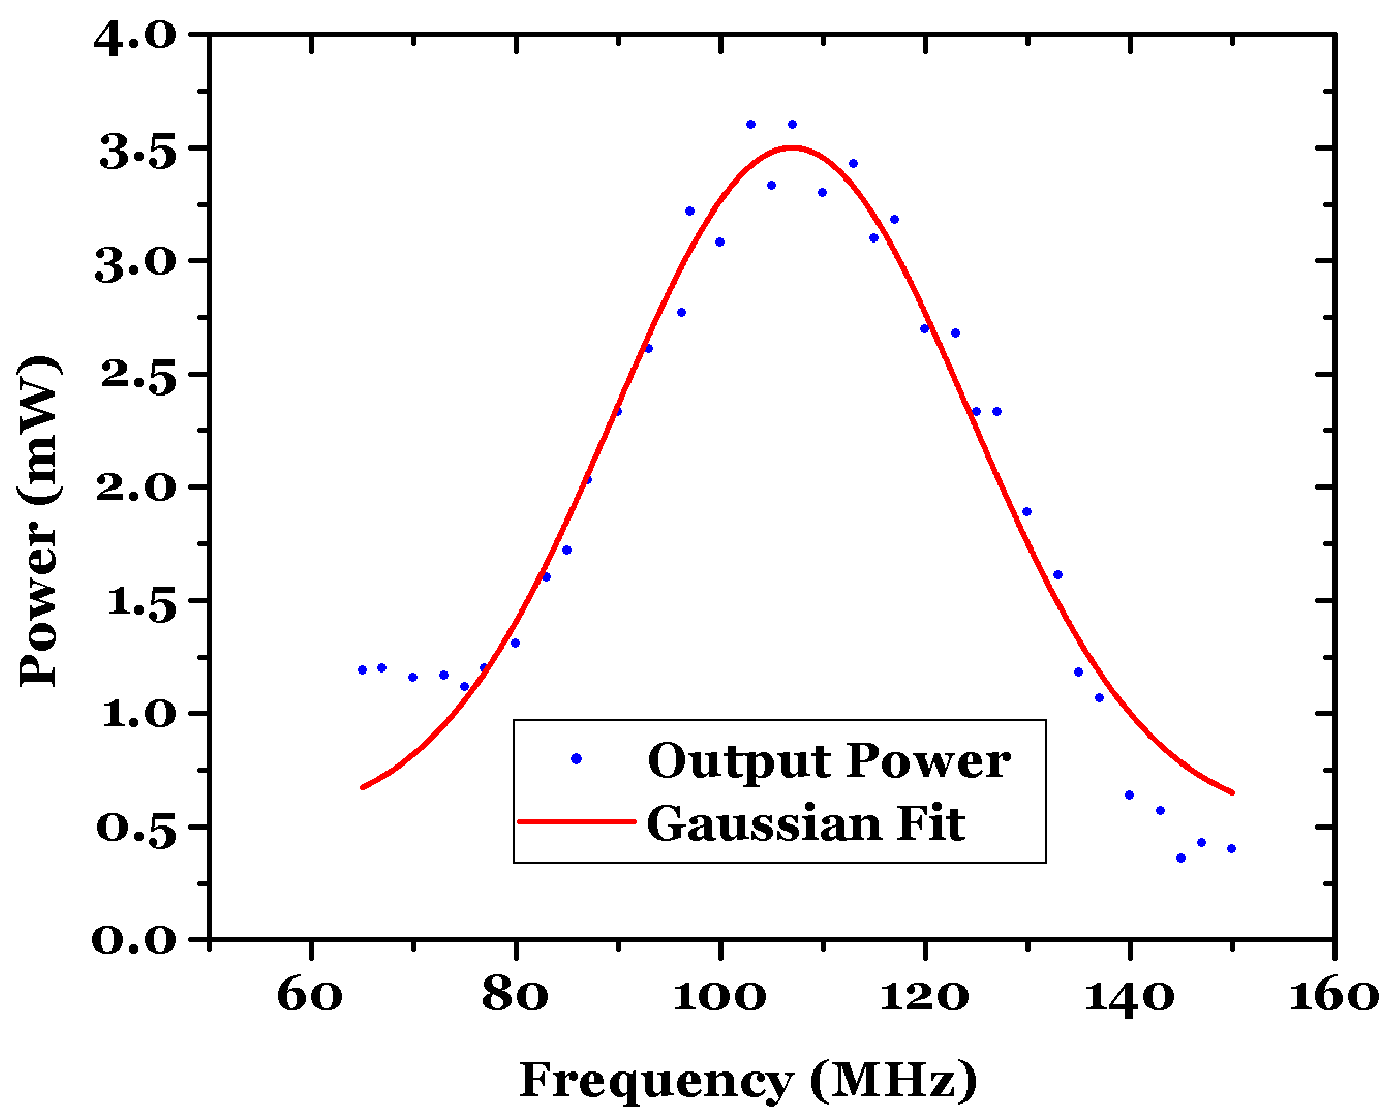
\includegraphics[height=2.5in]{figures/graph.png}
%
%    \caption[Optional: Short caption to appear in List of
%    Figures]{Full caption to appear below the Figure}
%
%    \label{figure1}
%\end{figure}

% +--------------------------------------------------------------------+
% |To create cross-references to figures, tables and segments
% |of text, LaTeX provides the following commands:
% |   \label{marker}
% |   \ref{marker}
% |   \pageref{marker}
% | where {marker} is a unique identifier.
% |
% | In the line above, we use \label{figure1} to mark a location
% | we wish to refer to later.  LATEX replaces \ref by the number of
% | the chapter, section, subsection, figure, or table after which the
% | corresponding \label command was issued. \pageref prints the page
% | number of the page where the \label command occurred.
% |
% +--------------------------------------------------------------------+

%See the file chapter1.tex for examples of the commands used to
%insert a figure or table, add a caption, etc.  Here is an example of
%a table:

%\begin{table}[ht]
%
%% +--------------------------------------------------------------------+
%% | We include the command \begin{center} to center the table
%% | horizontally on the page.  Note use of the command \end{center}
%% | to turn off centering after the table is defined.
%% +--------------------------------------------------------------------+
%    \begin{center}
%
%% +--------------------------------------------------------------------+
%% | The table is created with this command
%% |
%% | \begin{tabular}[pos]{table spec}
%% |
%% | The "pos" argument specifies the vertical position of the table
%% | relative to the baseline of the surrounding text.  Use t, b, or c
%% | to specify alignment at the top, bottom, or center.
%% |
%% | The "table spec" command defines the format of the table
%% |   l for a column of left-aligned text
%% |   r for a column of right-aligned text
%% |   c for centered text
%% |   p{width} for a column containing justified text with line breaks
%% |   | for a vertical line
%% |
%% |  In this example, the caption is made to appear above the table
%% |  by positioning the \caption command before the \begin{tabular
%% |  command. To position the caption below the table, insert the
%% |  \caption command after the \end{tabular} command.
%% +--------------------------------------------------------------------+
%    \caption{Caption to appear above the table}
%    \begin{tabular}[c]{|c|c|c|}
%        \hline
%        Column 1 Heading & Column 2 Heading & Column 3 Heading \\
%        \hline
%        Col 1 Row 1 & Col 2 Row 1 & Col 3 Row 1\\
%        Col 1 Row 2 & Col 2 Row 2 & Col 3 Row 2\\
%        Col 1 Row 3 & Col 2 Row 3 & Col 3 Row 3\\
%        \hline
%    \end{tabular}
%
%    \label{table1}
%   \end{center}
%\end{table}



% +--------------------------------------------------------------------+
% | Replace \section headings below with the title of your
% | subsections.  LaTeX will automatically number the subsections 1.1,
% | 1.2, 1.3, etc.
% +--------------------------------------------------------------------+

%\section{Making References to Figures or Tables}
%\label{makereference1.1}
%
%It is possible to create cross-references and hyperlinks to items or
%sections within your paper.  For example, here is a reference to
%Fig.~\ref{figure1} mentioned at the beginning of this chapter and a
%reference to the Table~\ref{table1}.
%
%\section{Making a Reference to a Chapter Subsection}
%\label{makereference1.2}
%
%In this section, we refer back to text mentioned in
%Section~\ref{makereference1.1} on page~\pageref{makereference1.1}.
%
%\section{Making a Citation}
%\label{makereference1.3}
%
%Here's an example of a citation to a single
%work.~\citep{CT:Weiner:1999} It's also possible to make multiple
%citations.~\citep{CT:Phillips:1985, ARP:Loy:1974}
%
%This template uses BibTeX to manage and format citations.  BibTeX is
%not the only way to create a bibliography within LaTeX, but it's
%generally considered to be the best option for long documents like a
%thesis or dissertation.~\citep{CT:Gould:1988}  There are a few more
%sample citations in this paragraph so you can see examples of how
%in-text references are made and how the bibliography is
%formatted.~\citep{ARP:Melinger:1991} See the file "BibTeX Guide.pdf"
%for information on how to use BibTeX.
